\chapter{정지작용과 오일러--라그랑주 방정식}

\lectureoverview{흔히 쓰는 \emph{최소 작용의 원리}라는 이름은 핵심을 가린다. 물리적 궤적에서 작용은 정지하지만, 반드시 최소가 되는 것은 아니다. 먼저 보통의 평형에서 이 명제를 이끌어 내고, 점에서 함수 전체로 확장한 뒤, 경로를 이산화해 오일러--라그랑주 방정식을 유도하고 뉴턴 방정식을 되찾겠다. 이어서 회전 좌표와 극좌표를 살펴보며 라그랑주 형식이 단순한 표기법의 변화 이상임을 알아보겠다.}

\section{최소가 아니라 정지}

전통적인 명칭에서 믿기 어려운 부분은 \emph{최소}라는 말이다. 고전역학적 궤적이 항상 작용을 최소로 만드는 것은 아니다. 가능한 궤적들의 공간에서 작용이 최대가 되거나 안장점에 이를 수도 있다. 올바른 원리는 작용이 \emph{정지값을 갖는다}는 것이다. 즉, 작용의 일차 변화가 사라진다.

먼저 더 간단한 평형 문제부터 살펴보자. 정지 상태를 유지하는 입자는 가속도가 없으므로 알짜힘은 사라져야 한다. 일차원 퍼텐셜에서 유도되는 힘이라면
\begin{equation}
  F(x)=-\frac{dV}{dx},
  \label{eq:force-from-v}
\end{equation}
평형 조건은 다음과 같다.
\begin{equation}
  \frac{dV}{dx}=0.
  \label{eq:stationary-v-one}
\end{equation}

\begin{figure}[htbp]
  \centering
  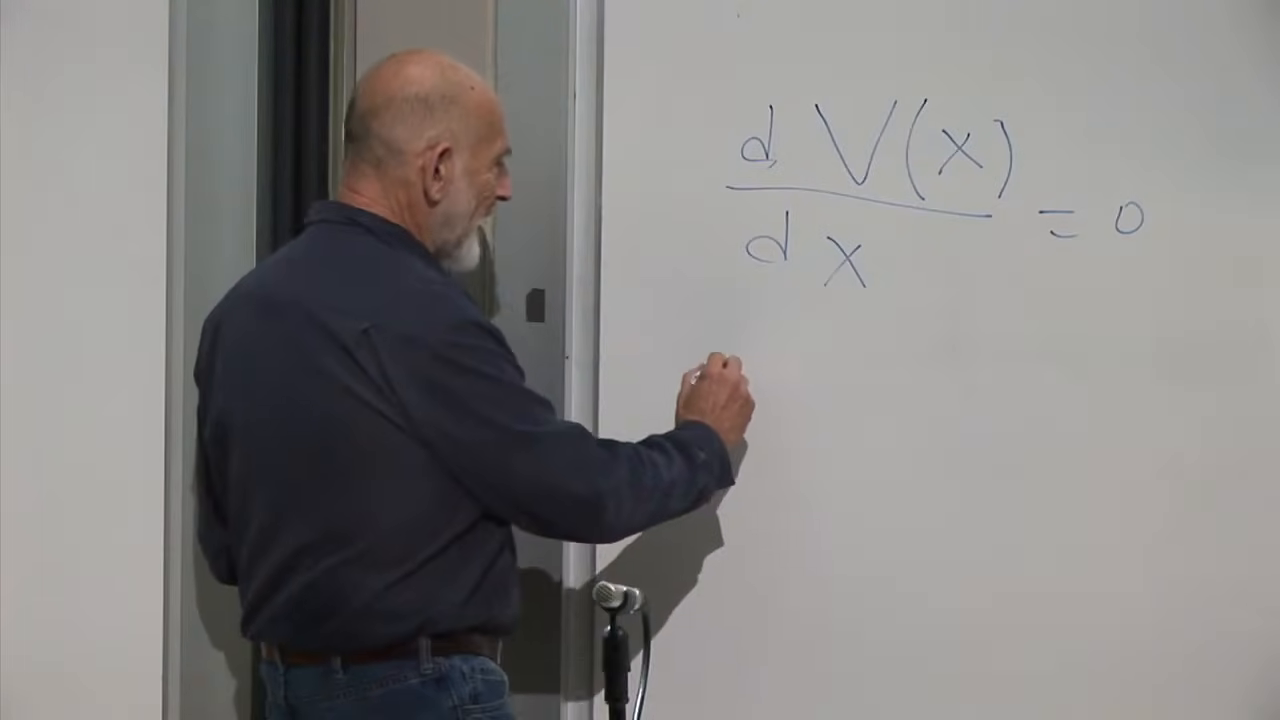
\includegraphics[width=0.74\textwidth]{lecture_03_figure_02.png}
  \caption{일차원 평형 조건: 퍼텐셜이 정지값을 갖는 곳에서 힘이 사라진다.}
  \lectureframe{00:02:51}
\end{figure}

이제 입자를 작은 양만큼 \(\delta x\)변위시켜 보자. 일차 근사에서는, \begin{equation}
  \delta V
  =V(x+\delta x)-V(x)
  =\frac{dV}{dx}\,\delta x+O(\delta x^2).
  \label{eq:first-variation-one}
\end{equation}평형 상태에서는 \(\delta x\)의 부호가 어느 쪽이든 선형항이 0이다.\begin{equation}
  \delta V=0
  \qquad\hbox{to first order.}
  \label{eq:delta-v-zero-one}
\end{equation}이는 유한하게 움직인 뒤에도 \(V\)가 정확히 변하지 않는다는 뜻이 아니다. 선도 변화가 이차 이상이라는 뜻이다. 최소와 최대 모두 이 조건을 만족한다.

\begin{figure}[htbp]
  \centering
  \begin{tikzpicture}[scale=0.95,>=Latex]
    \draw[->] (-0.2,0) -- (3.35,0) node[right] {$x$};
    \draw[->] (0,-0.2) -- (0,2.25) node[above] {$V$};
    \draw[blue!65!black,thick,smooth]
      plot coordinates {(0.2,1.85) (0.75,0.85) (1.55,0.35)
                        (2.35,0.85) (3.0,1.85)};
    \fill[red!65!black] (1.55,0.35) circle (2pt);
    \node at (1.55,-0.34) {minimum};
    \begin{scope}[xshift=4.25cm]
      \draw[->] (-0.2,0) -- (3.35,0) node[right] {$x$};
      \draw[->] (0,-0.2) -- (0,2.25) node[above] {$V$};
      \draw[blue!65!black,thick,smooth]
        plot coordinates {(0.2,0.35) (0.75,1.25) (1.55,1.85)
                          (2.35,1.25) (3.0,0.35)};
      \fill[red!65!black] (1.55,1.85) circle (2pt);
      \node at (1.55,-0.34) {maximum};
    \end{scope}
  \end{tikzpicture}
  \caption{정지 조건은 일차 미분값을 정할 뿐, 그 점이 최소인지 최대인지는 정하지 않는다.}
  \label{fig:min-max-stationary}
\end{figure}

여러 좌표 \(q_i\)에 대해서는 일차 변분이 다음과 같다.
\begin{equation}
  \delta V
  =\sum_i\frac{\partial V}{\partial q_i}\,\delta q_i.
  \label{eq:first-variation-many}
\end{equation}
이 값이 모든 독립적인 무한소 변위 \(\delta q_i\)에 대해 사라져야 한다면, 각 계수가 모두 사라져야 한다.
\begin{equation}
  \frac{\partial V}{\partial q_i}=0
  \qquad\hbox{for every }i.
  \label{eq:stationary-v-many}
\end{equation}

이차원 퍼텐셜은 롤러코스터보다는 기복이 있는 지형으로 떠올리는 편이 낫다. 정지점은 골짜기 바닥일 수도, 언덕 꼭대기일 수도, 안장점일 수도 있다. 안장점에서는 한 방향으로는 처음에 올라가고 다른 방향으로는 처음에 내려간다. 따라서 그 점에서 모든 일차 미분이 사라지더라도, 복원 거동은 한 방향에서는 안정적이고 다른 방향에서는 불안정할 수 있다.

\begin{figure}[htbp]
  \centering
  \includegraphics[width=0.76\textwidth]{lecture_03_figure_06.png}
  \caption{안장점에서는 모든 방향의 일차 변화가 사라지지만, 그 점에서 이웃한 변위는 한 축을 따라 올라가고 다른 축을 따라 내려간다.}
  \lectureframe{00:08:20}
\end{figure}

좌표가 많은 공간에서는 순수한 최대나 최소보다 안장점이 더 흔하다. 그래서 \emph{정지}라는 말이 오래도록 정확하게 쓰인다. 다음 조건은 \begin{equation}
  \delta V=0
  \label{eq:equilibrium-variation}
\end{equation}이차 거동을 미리 단정하지 않으면서 평형을 요약한다.

\section{점에서 함수로}

역학은 고립된 평형점이 아니라 운동 전체를 다룬다. 궤적은 \(x(t)\)와 같은 함수이거나, \((x(t),y(t),z(t))\)와 같은 함수들의 모음이다. 함수 전체를 변화시켜 어떤 양을 정지시키는 수학적 문제를 \emph{변분법}이라 한다. 운동에 적용하기 전에 더 간단한 예 세 가지를 살펴보자.

\subsection{최단 곡선과 측지선}

평면에 두 점을 고정하고, 두 점을 잇는 곡선을 \(y(x)\)로 나타내자. 짧은 구간에서, \begin{equation}
  ds=\sqrt{dx^2+dy^2}
  =dx\sqrt{1+\left(\frac{dy}{dx}\right)^2},
  \label{eq:line-element}
\end{equation}마지막 식은 \(dx>0\)이라고 가정한 것이다. 전체 길이는 다음 범함수로 주어진다.\begin{equation}
  S[y]=\int_{x_0}^{x_1}
  \sqrt{1+y'(x)^2}\,dx.
  \label{eq:arc-length-functional}
\end{equation}대괄호는 \(S\)가 함수 전체를 입력으로 받는다는 점을 강조한다. 양 끝점을 고정한 채 곡선을 조금씩 바꿨을 때 \begin{equation}
  \delta S=0
  \label{eq:stationary-length}
\end{equation}를 만족하는 곡선은 직선이다.

\begin{figure}[htbp]
  \centering
  \includegraphics[width=0.78\textwidth]{lecture_03_figure_07.png}
  \caption{고정된 두 끝점을 잇는 시험 곡선. 곡선의 길이는 미소 빗변 \(ds\)들을 더한 값이다.}
  \lectureframe{00:13:36}
\end{figure}

같은 문제를 곡면에서도 생각할 수 있다. 두 말뚝 사이에 줄을 팽팽히 당기면 제약된 경로 중 가장 짧은 경로를 물리적으로 떠올릴 수 있다. 길이가 정지하는 이런 곡선을 \emph{측지선}이라 한다. 평면에서는 직선이지만, 구면이나 굴곡진 표면에서는 대체로 직선이 아니다.

\subsection{페르마의 원리}

위치에 따라 속력이 달라지는 매질에서 빛은 \(c(x,y)\)공간상 최단 경로를 따르지 않을 수도 있다. 짧은 구간을 지나는 데 걸리는 시간은 거리를 그 지점의 속력으로 나눈 값이므로, \begin{equation}
  T[y]
  =\int_{x_0}^{x_1}
  \frac{\sqrt{1+y'(x)^2}}{c(x,y)}\,dx.
  \label{eq:fermat-functional}
\end{equation}페르마의 원리에 따르면 \begin{equation}
  \delta T=0.
  \label{eq:fermat-stationary}
\end{equation}이다. \(c\)가 일정하면 이 문제는 최단 거리 문제로 환원된다. 하지만 굴절률이 위치에 따라 변하는 매질에서는 최단 거리와 국소적인 전파 속력 사이의 균형으로 가장 빠른 경로가 정해진다.

\begin{figure}[htbp]
  \centering
  \includegraphics[width=0.80\textwidth]{lecture_03_figure_08.png}
  \caption{빛의 국소 속력이 위치에 따라 달라지는 매질에서 광선의 최소 시간 범함수.}
  \lectureframe{00:22:50}
\end{figure}

시사적인 농담에서는 당시 이탈리아에서 중성미자가 이례적으로 빠르게 움직였다는 최근 주장을 언급한다. 물리학적 논의는 곧 믿을 만한 예로 돌아온다. 보통의 빛은 굴절률에 따라 물질 속에서 속력이 달라진다.

\subsection{매달린 사슬}

두 점에 고정된 사슬은 현수선 형태로 놓인다. 사슬의 각 미소 부분은 중력 퍼텐셜 에너지에 기여하므로, 전체 퍼텐셜 에너지도 사슬을 따라 적분한 값이다. 여기서도 양 끝점은 고정되어 있고, 미지의 모양은 함수이며, 적분값은 정지해야 한다.

\begin{figure}[htbp]
  \centering
  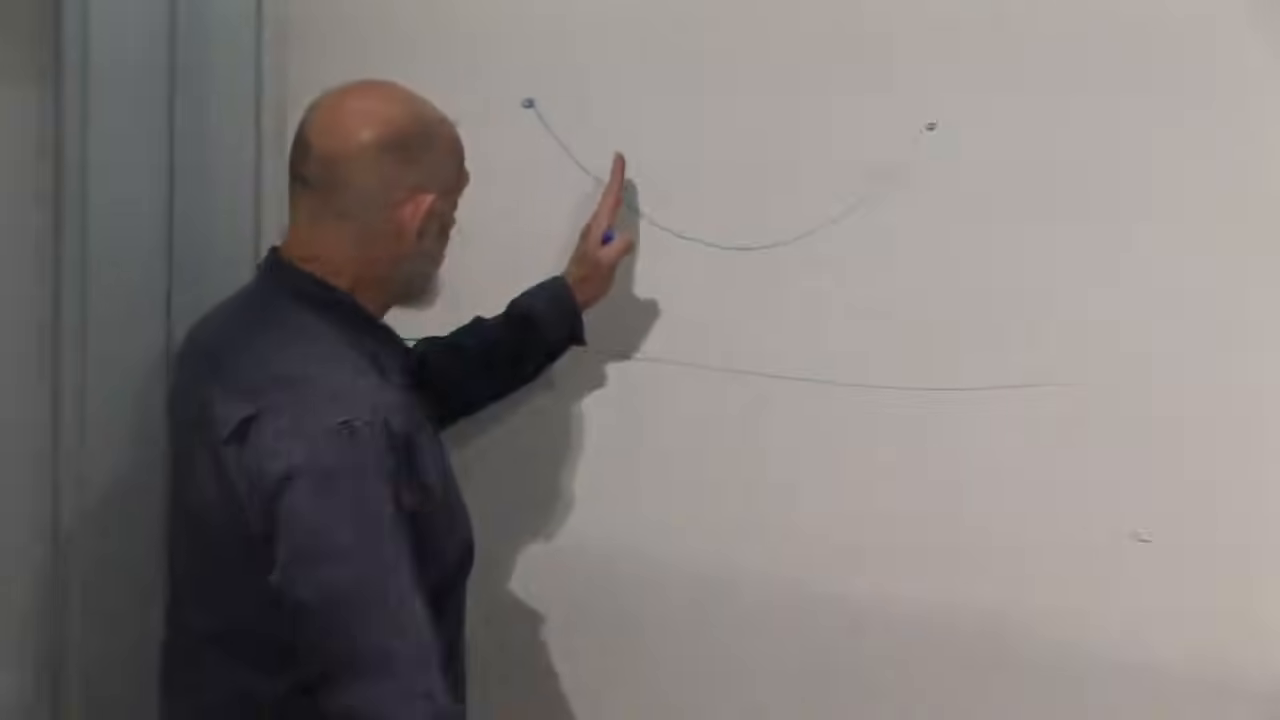
\includegraphics[width=0.76\textwidth]{lecture_03_figure_03.png}
  \caption{고정된 지지점 사이에 매달린 사슬. 정지 모양은 전체 중력 퍼텐셜 에너지로 결정된다.}
  \lectureframe{00:30:41}
\end{figure}

이 예들은 같은 구조를 갖는다. 양 끝점이 고정되어 있고, 그 사이에 함수가 있으며, 그 함수의 적분에 대한 일차 변분이 사라진다. 이처럼 전체에 주어진 조건을 미분방정식으로 바꾸는 것이 변분 문제를 푼다는 뜻이다.

\section{경계값 문제로서의 역학}

\(t\)가 독립변수이므로 궤적은 흔히 시간을 가로축으로 그린다. 그런데 물리학에는 시간을 위쪽으로 그리는 강한 관습도 있다. 한 일화에 따르면, 젊은 시절부터 노년까지의 그림을 순서대로 배열하게 하는 실험에서 글을 왼쪽에서 오른쪽으로 읽는 사람들은 그림도 왼쪽에서 오른쪽으로 배열하는 경향이 있었고, 오른쪽에서 왼쪽으로 읽는 사람들은 그 반대로, 세로쓰기에 익숙한 사람들은 세로로 배열하는 경향이 있었다. 농담의 결론은 물리학자들이야말로 시간이 위쪽으로 흐른다고 우기는 사람들이라는 것이다. 여기서는 관례에 따라 \(t\)축을 가로로 두겠다. 그러면 \(x(t)\)를 그래프로 자연스럽게 나타낼 수 있기 때문이다.

초기값 정식화에서는 \(t_0\)에서의 자료가 다음과 같다.\begin{equation}
  x(t_0)=x_0,
  \qquad
  \dot x(t_0)=v_0.
  \label{eq:initial-value-data}
\end{equation}그러면 뉴턴 방정식이 그 이후의 궤도를 결정한다. 변분 정식화는 다른 문제를 제기한다. 두 끝점 사건을 \begin{equation}
  x(t_0)=x_0,
  \qquad
  x(t_1)=x_1,
  \label{eq:boundary-value-data}
\end{equation}로 지정하고 그 사이의 물리적 경로를 구하는 것이다. 초기 속도는 더 이상 주어지지 않으며, 해의 일부로 결정된다.

\begin{figure}[htbp]
  \centering
  \includegraphics[width=0.76\textwidth]{lecture_03_figure_09.png}
  \caption{역학적 궤적 \(x(t)\). 한쪽 끝에서 위치와 기울기를 지정할 수도 있고, 두 끝점 시각에서 위치를 지정할 수도 있다.}
  \lectureframe{00:27:41}
\end{figure}

정지시킬 양은 \emph{작용}이다. \begin{equation}
  A[x]=\int_{t_0}^{t_1}L(x,\dot x,t)\,dt.
  \label{eq:action-one}
\end{equation}적분함수 \(L\)를 \emph{라그랑지안}이라 한다. 라그랑지안은 위치와 속도에 의존하며, 시간에 명시적으로 의존할 수도 있다. 작용 원리는 다음과 같다. \begin{equation}
  \delta A=0
  \label{eq:stationary-action}
\end{equation}끝점 조건 \begin{equation}
  \delta x(t_0)=\delta x(t_1)=0.
  \label{eq:fixed-endpoint-variations}
\end{equation}을 만족하는 모든 작은 경로 변분에 대해 성립한다. 끝점 조건은 필수적이다. 같은 두 사건을 잇는 이웃한 경로끼리 비교하기 때문이다.

\section{이산화에 따른 오일러--라그랑주 방정식의 유도}

작용은 경로의 무한히 많은 값에 의존하는 범함수다. 변분을 구체적으로 다루기 위해 시간 구간을 길이 \(\epsilon\)인 단계들로 나누자. \begin{equation}
  t_n=t_0+n\epsilon,
  \qquad
  x_n=x(t_n),
  \label{eq:discrete-times}
\end{equation}그리고 \(n\)번째 구간의 속도를 다음과 같이 근사한다. \begin{equation}
  v_n=\frac{x_{n+1}-x_n}{\epsilon}.
  \label{eq:discrete-velocity}
\end{equation}그러면 적분은 보통의 합으로 바뀐다. \begin{equation}
  A_\epsilon
  =\sum_{n=0}^{N-1}
  \epsilon L\left(x_n,\frac{x_{n+1}-x_n}{\epsilon}\right).
  \label{eq:discrete-action}
\end{equation}\(n\)는 시간 구간의 첨자이고, 뒤에서 공간 좌표와 입자를 나타내는 \(i\)를 쓸 수 있도록 이 표기를 택했다.

\begin{figure}[htbp]
  \centering
  \includegraphics[width=0.82\textwidth]{lecture_03_figure_10.png}
  \caption{시간 구간들로 대체한 궤적. 내부의 한 점을 변분하면 그 양옆 구간만 바뀐다.}
  \lectureframe{00:38:30}
\end{figure}

다른 모든 \(x_k\)를 고정한 채 내부의 한 점 \(x_n\)만 변분하자. 합에서 \(x_n\)에 의존하는 항은 두 개뿐이다. \begin{align}
  A_\epsilon\big|_{x_n}
  &=
  \epsilon L\left(x_n,\frac{x_{n+1}-x_n}{\epsilon}\right)
  \notag\\
  &\quad+
  \epsilon L\left(x_{n-1},
                  \frac{x_n-x_{n-1}}{\epsilon}\right).
  \label{eq:two-neighbor-terms}
\end{align}미분하면 다음을 얻는다. \begin{align}
  0=\frac{\partial A_\epsilon}{\partial x_n}
  &=
  \epsilon\frac{\partial L_n}{\partial x_n}
  -\frac{\partial L_n}{\partial v_n}
  +\frac{\partial L_{n-1}}{\partial v_{n-1}}.
  \label{eq:discrete-el-variation}
\end{align}부호가 반대인 데에는 간단한 기하학적 이유가 있다. \(x_n\)를 높이면 뒤쪽 구간의 기울기는 커지고 앞쪽 구간의 기울기는 작아진다.

\begin{figure}[htbp]
  \centering
  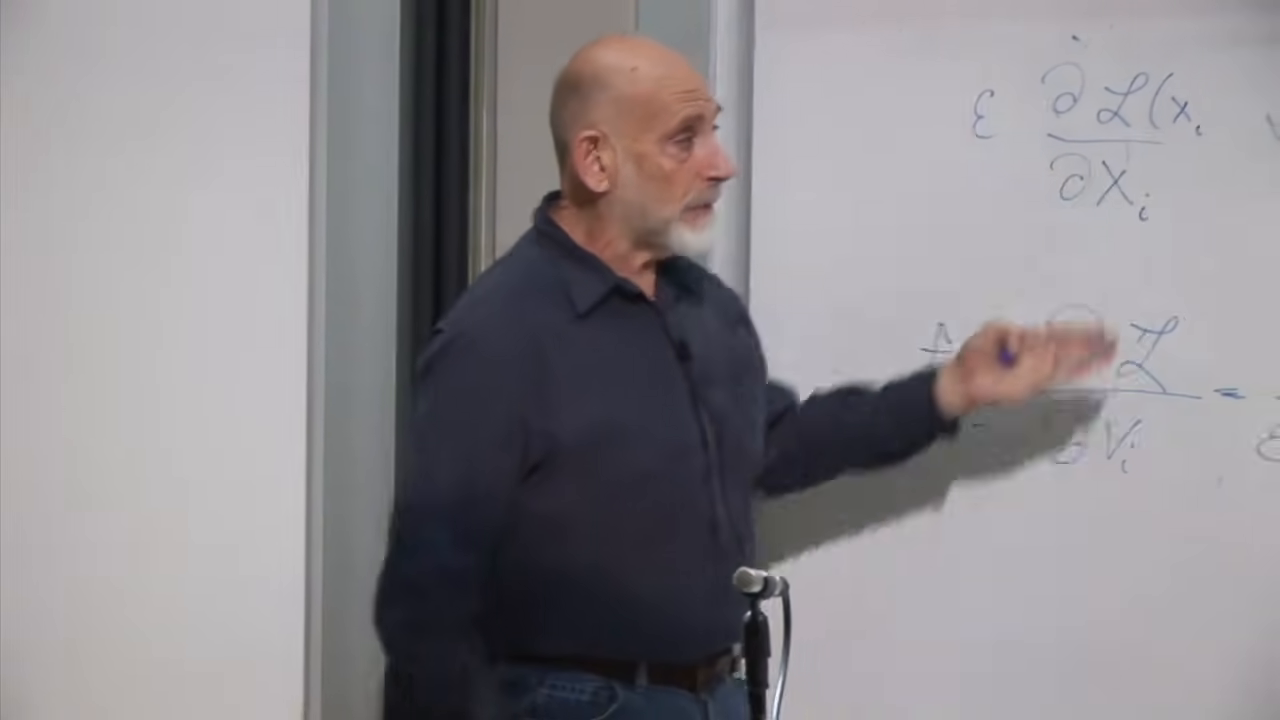
\includegraphics[width=0.74\textwidth]{lecture_03_figure_04.png}
  \caption{위치에 대한 직접 미분항과 양옆 구간의 속도 미분에서 오는 두 기여.}
  \lectureframe{00:45:26}
\end{figure}

식~\eqref{eq:discrete-el-variation}을 정리하면 다음과 같다. \begin{equation}
  \frac{1}{\epsilon}
  \left(
    \frac{\partial L_n}{\partial v_n}
    -\frac{\partial L_{n-1}}{\partial v_{n-1}}
  \right)
  =
  \frac{\partial L_n}{\partial x_n}.
  \label{eq:discrete-el}
\end{equation}왼쪽은 이웃한 두 값의 차분몫이다. \(\epsilon\to0\)가 되면 꺾은선은 매끄러운 경로가 되고, 차분몫은 시간 미분으로 바뀐다. \begin{equation}
  \boxed{
  \frac{d}{dt}\left(\frac{\partial L}{\partial\dot x}\right)
  =
  \frac{\partial L}{\partial x}}
  .
  \label{eq:euler-lagrange-one}
\end{equation}이것이 오일러--라그랑주 방정식이다.

\begin{figure}[htbp]
  \centering
  \includegraphics[width=0.78\textwidth]{lecture_03_figure_11.png}
  \caption{모든 내부 시간 구간에서 정지 조건을 적용해 얻은 완성된 오일러--라그랑주 방정식.}
  \lectureframe{00:49:25}
\end{figure}

\(L\)가 주어지면 식~\eqref{eq:euler-lagrange-one}은 일종의 기계처럼 작동한다. 주어진 함수를 미분하면 경로에 대한 미분방정식이 나온다.

\begin{classroomqa}\audiencequestion{오일러--라그랑주 결과는 \(x\)와 \(\dot x\)의 임의의 함수에 대해 성립하나요?\lecturetimestamp{00:49:37--00:50:24}}\lecturerresponse{미분에 필요한 정칙성 조건이 충족되면 성립합니다. 독립변수 \(x\)가 \(t\)의 역할을 하고 미지 함수 \(y(x)\)가 \(x(t)\)의 역할을 하도록 바꾸어 쓰면, 호의 길이 예제도 정확히 같은 형식입니다. 그 경우 오일러--라그랑주 방정식의 해는 직선입니다.}\end{classroomqa}

\section{라그랑지안으로부터 뉴턴 방정식 유도하기}

퍼텐셜 \(V(x)\) 속에서 직선 운동하는 입자에 대해 다음을 택하자. \begin{equation}
  L(x,\dot x)=T-V
  =\frac12m\dot x^2-V(x).
  \label{eq:lagrangian-tv-one}
\end{equation}전체 에너지가 \(T+V\)이므로 마이너스 부호가 이상해 보일 수 있다. 하지만 라그랑지안은 에너지가 아니다. 오일러--라그랑주 방정식이 올바른 운동을 내놓는지가 판별 기준이다. 부호를 두고 모의 투표를 하자는 제안은 받아들이지 않는다. 답은 투표로 정하는 것이 아니라 확인해야 한다.

먼저, \begin{equation}
  \frac{\partial L}{\partial\dot x}=m\dot x.
  \label{eq:conjugate-momentum-one}
\end{equation}이것은 운동량이다. 더 일반적으로 좌표 \(q\)에 켤레인 운동량은 다음과 같이 정의한다. \begin{equation}
  p_q=\frac{\partial L}{\partial\dot q}.
  \label{eq:conjugate-momentum-general}
\end{equation}식~\eqref{eq:conjugate-momentum-one}을 시간에 대해 미분하면 \(m\ddot x\)을 얻고, \begin{equation}
  \frac{\partial L}{\partial x}
  =-\frac{dV}{dx}.
  \label{eq:lagrangian-position-derivative}
\end{equation}가 성립한다. 따라서 오일러--라그랑주 방정식은 \begin{equation}
  m\ddot x=-\frac{dV}{dx}=F(x),
  \label{eq:newton-from-action}
\end{equation}이 되며, 이것이 뉴턴의 제이 법칙이다.

\begin{figure}[htbp]
  \centering
  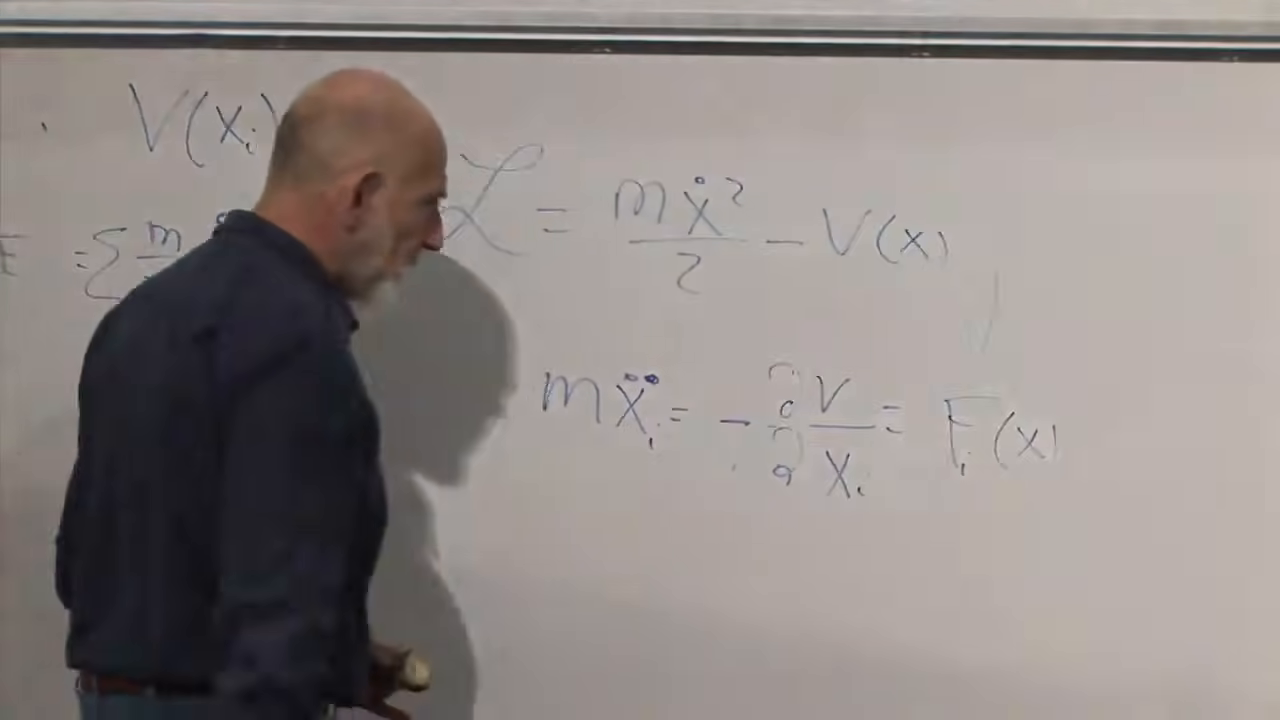
\includegraphics[width=0.80\textwidth]{lecture_03_figure_05.png}
  \caption{운동 에너지, 퍼텐셜 에너지, \(L=T-V\), 그리고 되찾은 뉴턴 방정식의 성분별 표현을 한 판에 나타냈다.}
  \lectureframe{00:57:52}
\end{figure}

좌표가 여러 개 \(q_i\)이면, \begin{equation}
  L(\mathbf q,\dot{\mathbf q})
  =\sum_i\frac12m_i\dot q_i^{\,2}-V(q_1,q_2,\ldots),
  \label{eq:lagrangian-tv-many}
\end{equation}좌표마다 방정식이 하나씩 있다. \begin{equation}
  \frac{d}{dt}\left(\frac{\partial L}{\partial\dot q_i}\right)
  =\frac{\partial L}{\partial q_i}
  \quad\Longrightarrow\quad
  m_i\ddot q_i=-\frac{\partial V}{\partial q_i}=F_i.
  \label{eq:euler-lagrange-many}
\end{equation}궤적은 여전히 하나의 곡선이지만, 이제 고차원 배치 공간을 지난다.

\begin{classroomqa}\audiencequestion{뉴턴 법칙에서 역으로 출발해 답을 재현하는 범함수를 고안한 것뿐인가요?\lecturetimestamp{00:58:07--01:00:04}}\lecturerresponse{그렇게 보는 것은 생산적인 관점이 아닙니다. 라그랑지안은 물리계를 간결하게 규정합니다. 모든 좌표와 속도를 포함하는 하나의 함수에 운동 방정식 전체를 담습니다. 새로운 이론에서는 물리학자들이 각 방정식을 따로 추측하기보다 보통 작용을 제안하고 방정식을 유도합니다.}\end{classroomqa}

이런 통합은 한 가지 장점이다. 좌표 선택의 자유도 또 다른 장점이다. 직선이 최단이라는 명제는 평면을 데카르트 좌표, 극좌표 또는 곡선 좌표 중 무엇으로 기술하는지에 좌우되지 않는다. 마찬가지로 작용의 정지 조건도 좌표에 무관하지만, \(L\)의 식과 그에 따른 성분 방정식은 좌표에 따라 달라진다.

\section{회전목마에서 본 자유 입자}

\((x,y)\)를 관성계의 데카르트 좌표, \((X,Y)\)를 각속도 \(\omega\)로 균일하게 회전하는 좌표라고 하자. 여기서 사용한 방향 규약에 따르면, \begin{align}
  x&=X\cos\omega t+Y\sin\omega t,
  \notag\\
  y&=-X\sin\omega t+Y\cos\omega t.
  \label{eq:rotating-coordinate-map}
\end{align}두 좌표계 사이의 각도는 \(\omega t\)이다.

\begin{figure}[htbp]
  \centering
  \includegraphics[width=0.76\textwidth]{lecture_03_figure_12.png}
  \caption{관성계의 데카르트 좌표축과 균일 회전하는 좌표축. 같은 점도 회전 좌표계에서는 시간에 따라 변하는 좌표를 갖는다.}
  \lectureframe{01:06:05}
\end{figure}

자유 입자의 관성계 라그랑지안은 다음과 같다. \begin{equation}
  L_{\mathrm{in}}
  =\frac{m}{2}\left(\dot x^2+\dot y^2\right).
  \label{eq:free-inertial-lagrangian}
\end{equation}식~\eqref{eq:rotating-coordinate-map}을 미분하고 \(\sin^2\omega t+\cos^2\omega t=1\)를 이용하자. 삼각함수 항들을 합하면 \begin{align}
  \dot x^2+\dot y^2
  &=
  \dot X^2+\dot Y^2\\
  &\quad+\omega^2(X^2+Y^2)\\
  &\quad+2\omega(Y\dot X-X\dot Y).
  \label{eq:rotating-speed}
\end{align}가 된다. 따라서 \begin{align}
  L_{\mathrm{rot}}
  &=
  \frac{m}{2}(\dot X^2+\dot Y^2)\\
  &\quad+\frac{m\omega^2}{2}(X^2+Y^2)\\
  &\quad+m\omega(Y\dot X-X\dot Y).
  \label{eq:rotating-lagrangian}
\end{align}이다.

\begin{figure}[htbp]
  \centering
  \includegraphics[width=0.84\textwidth]{lecture_03_figure_13.png}
  \caption{변환된 자유 입자 라그랑지안: 보통의 운동 에너지, 이차 원심력 항, 속도에 선형인 항.}
  \lectureframe{01:12:16}
\end{figure}

좌표에 대한 이차항은 \(-V_{\mathrm{fict}}\)의 형태이며, 여기서 \begin{equation}
  V_{\mathrm{fict}}
  =-\frac{m\omega^2}{2}(X^2+Y^2).
  \label{eq:centrifugal-potential}
\end{equation}이다. 이 항은 바깥쪽으로 갈수록 작아지므로 원심력 \(m\omega^2(X,Y)\)을 만들어 낸다.

식~\eqref{eq:rotating-lagrangian}의 마지막 항은 좌표와 속도 모두에 선형이다. 오일러--라그랑주 방정식을 적용하면 \begin{align}
  m\ddot X&=m\omega^2X-2m\omega\dot Y,
  \notag\\
  m\ddot Y&=m\omega^2Y+2m\omega\dot X.
  \label{eq:rotating-equations}
\end{align}를 얻는다. \(\omega^2\)에 비례하는 항은 원심력에 해당하고, 속도에 비례하는 항은 코리올리 힘에 해당한다. 회전 평면 안에서 벡터로 쓰면 \begin{equation}
  \mathbf F_{\mathrm{C}}
  =-2m\,\boldsymbol\omega\times\mathbf v_{\mathrm{rot}},
  \label{eq:coriolis-vector}
\end{equation}이며, 반대 방향 규약을 택하면 부호를 조정해야 한다.

\begin{figure}[htbp]
  \centering
  \includegraphics[width=0.84\textwidth]{lecture_03_figure_14.png}
  \caption{회전 좌표계의 방정식. 좌표에 비례하는 항은 원심 가속도를, 속도 성분 간 교차항은 코리올리 가속도를 만든다.}
  \lectureframe{01:20:20}
\end{figure}

핵심은 대수 계산이 사라진다는 것이 아니다. 하나의 스칼라 함수에 좌표 변환을 적용하면 서로 결합된 두 방정식과 두 가상력이 모두 나온다는 점이다.

\begin{classroomqa}\audiencequestion{이 방법은 곡선 좌표가 아무리 복잡해도 쓸 수 있나요?\lecturetimestamp{01:22:01--01:22:17}}\lecturerresponse{그렇습니다. 새 좌표는 곡선 좌표여도 되고, 회전 좌표처럼 시간에 명시적으로 의존해도 됩니다. 작용을 새 변수로 다시 쓴 다음 같은 오일러--라그랑주 규칙을 적용하면 됩니다.}\end{classroomqa}

\section{극좌표와 순환 각도}

보통의 극좌표에서는, \begin{equation}
  x=r\cos\theta,
  \qquad
  y=r\sin\theta.
  \label{eq:polar-map}
\end{equation}\(r\)와 \(\theta\)는 모두 시간에 따라 변할 수 있다. 미분한 다음 제곱을 더하면 \begin{equation}
  \dot x^2+\dot y^2
  =\dot r^2+r^2\dot\theta^2.
  \label{eq:polar-speed}
\end{equation}를 얻는다. 중심 퍼텐셜 \(V(r)\)에 대해서는, \begin{equation}
  L
  =\frac{m}{2}\left(\dot r^2+r^2\dot\theta^2\right)-V(r).
  \label{eq:polar-lagrangian}
\end{equation}이다.

\begin{figure}[htbp]
  \centering
  \includegraphics[width=0.80\textwidth]{lecture_03_figure_15.png}
  \caption{극좌표의 기하학과 운동 에너지를 방사 운동 및 각운동으로 분해한 모습.}
  \lectureframe{01:23:30}
\end{figure}

방사 방향 방정식은 다음과 같다. \begin{equation}
  m\ddot r
  =mr\dot\theta^2-\frac{dV}{dr}.
  \label{eq:radial-equation}
\end{equation}첫 번째 항은 입자 자체의 각운동과 관련된 바깥쪽 원심력 기여다.

각도에 대해서는, \begin{equation}
  \frac{d}{dt}\left(\frac{\partial L}{\partial\dot\theta}\right)
  =\frac{\partial L}{\partial\theta}=0,
  \label{eq:theta-el}
\end{equation}중심 퍼텐셜이 \(\theta\)에 명시적으로 의존하지 않기 때문이다. 따라서 \begin{equation}
  \frac{d}{dt}\left(mr^2\dot\theta\right)=0,
  \qquad
  mr^2\dot\theta=\ell,
  \label{eq:angular-momentum}
\end{equation}이며, \(\ell\)는 보존되는 각운동량이다.

\begin{figure}[htbp]
  \centering
  \includegraphics[width=0.82\textwidth]{lecture_03_figure_16.png}
  \caption{각도에 대한 오일러--라그랑주 방정식의 우변은 0이며, 이에 따라 \(mr^2\dot\theta\)의 보존이 드러난다.}
  \lectureframe{01:29:25}
\end{figure}

각도 방정식에서 \begin{equation}
  \dot\theta=\frac{\ell}{mr^2}.
  \label{eq:theta-dot-angular-momentum}
\end{equation}를 얻는다. 이를 식~\eqref{eq:radial-equation}에 대입하면 \(r\)에 대한 방정식 하나만 남는다. \begin{equation}
  m\ddot r
  =\frac{\ell^2}{mr^3}-\frac{dV}{dr}.
  \label{eq:effective-radial-equation}
\end{equation}

\(L\)에서 빠져 있는 좌표를, 그 좌표가 각도가 아니더라도 관례적으로 \emph{순환} 좌표라고 부른다. \(q\)가 순환 좌표이면 \begin{equation}
  \frac{\partial L}{\partial q}=0
  \quad\Longrightarrow\quad
  \frac{d}{dt}\left(\frac{\partial L}{\partial\dot q}\right)=0.
  \label{eq:cyclic-conservation}
\end{equation}이다. 그 켤레 운동량은 보존된다. 이는 대칭성과 보존 법칙 사이의 일반적인 연결을 엿보게 해 준다.

\section{의미, 에너지, 적용 범위에 관한 질문}

이어지는 질문들은 이 형식론의 더 깊은 내용이 어디에 있는지 드러낸다.

\begin{classroomqa}\audiencequestion{라그랑지안이 올바른 고전 방정식을 준다는 사실을 발견하는 것 외에, 라그랑지안을 도출할 독립적인 근거가 있나요?\lecturetimestamp{01:33:25--01:35:07}}\lecturerresponse{역사적으로 한 세기가 넘는 고전역학의 발전을 통해 입자와 파동, 전자기장이 모두 이 형식으로 나타날 수 있음이 밝혀졌습니다. 고전적인 수준에서 이처럼 축적된 성공은 자연 법칙이 구성되는 방식에 관한 경험적 사실입니다. 더 깊은 설명은 양자역학에서 나오며, 그 논의는 뒤로 미루겠습니다.}\end{classroomqa}

\begin{classroomqa}\audiencequestion{회전 좌표계 라그랑지안에서 속도에 선형인 항에 보통의 운동 에너지나 퍼텐셜 에너지라는 해석을 붙일 수 있나요?\lecturetimestamp{01:35:08--01:36:23}}\lecturerresponse{아니요. 시간 병진에 대응하는 보존량은 해밀토니안 구성으로 구합니다. \(L\)의 모든 항을 운동 에너지나 퍼텐셜 에너지로 읽어 내는 것이 아닙니다. 식~\eqref{eq:rotating-lagrangian}에서는 속도에 선형인 항이 \(\sum_a\dot q_a\,\partial L/\partial\dot q_a-L\)에서 상쇄됩니다. 해밀토니안 형식에서는 이를 체계적으로 다룰 것입니다.}\end{classroomqa}

실제로 \(L_{\mathrm{rot}}\)는 시간에 명시적으로 의존하지 않으므로 \begin{equation}
  \begin{aligned}
    H_{\mathrm{rot}}
    &=\dot X\frac{\partial L}{\partial\dot X}
     +\dot Y\frac{\partial L}{\partial\dot Y}-L\\
    &=\frac{m}{2}(\dot X^2+\dot Y^2)
     -\frac{m\omega^2}{2}(X^2+Y^2)
  \end{aligned}
  \label{eq:rotating-hamiltonian-preview}
\end{equation}가 보존된다. 이것은 회전 좌표계의 자코비 적분이며, 관성계 관찰자가 부여하는 에너지와 수치상 같은 양은 아니다. 시간 의존적인 좌표 변환을 거치면 에너지의 수치적 형태가 보존되지 않을 수 있다.

\begin{classroomqa}\audiencequestion{중력 때문에 궤적이 휘어진다면 어떻게 하나요?\lecturetimestamp{01:36:30--01:37:10}}\lecturerresponse{뉴턴 중력이라면 중심력 라그랑지안에 \(V(r)=-GMm/r\)를 쓰면 됩니다. 휘어진 시공간은 일반상대론에 속하며 여기서는 전제하지 않습니다.}\end{classroomqa}

\begin{classroomqa}\audiencequestion{원심 퍼텐셜과 그 에너지는 그저 가상적인 것인가요?\lecturetimestamp{01:37:13--01:40:14}}\lecturerresponse{회전하는 플랫폼의 관찰자는 유효 힘을 측정하며 회전 좌표계의 보존량을 일관되게 사용할 수 있습니다. \emph{가상적}이라는 말은 이 항들이 비관성계 기술에서 생겨난다는 뜻이지, 관찰되는 효과가 허상이라는 뜻이 아닙니다. 에너지 자체는 일반적인 시간 의존 좌표 변환에서 불변량이 아닙니다.}\end{classroomqa}

\begin{classroomqa}\audiencequestion{속도에 의존하는 코리올리 힘은 어느 방향을 향하나요?\lecturetimestamp{01:40:22--01:42:36}}\lecturerresponse{회전 좌표계에서의 속도에 수직이며, 크기는 속력과 좌표계의 각속도에 비례합니다. 평면에서는 식\(\dot X\)과 \(\dot Y\)가 서로 반대 부호로 바뀌며, 식~\eqref{eq:rotating-equations}과 같습니다.}\end{classroomqa}

\begin{figure}[htbp]
  \centering
  \includegraphics[width=0.76\textwidth]{lecture_03_figure_17.png}
  \caption{속도 성분 간 교차항의 형태: 코리올리 힘은 회전 좌표계에서의 속도에 수직이다.}
  \lectureframe{01:41:40}
\end{figure}

\begin{classroomqa}\audiencequestion{출발점이 되는 라그랑지안은 반드시 관성계에서 써야 하나요?\lecturetimestamp{01:42:37--01:44:00}}\lecturerresponse{보통의 자유 입자에서는 뉴턴의 관성계 법칙이 간단한 출발 형태 \(m(\dot x^2+\dot y^2)/2\)를 줍니다. 이 물리 법칙을 알고 있다면 작용을 다른 어떤 좌표로도 변환할 수 있습니다. 회전 좌표계에서도 똑같이 간단한 운동 에너지 식을 쓸 수 있다고 독립적으로 가정해서는 안 됩니다.}\end{classroomqa}

자기장 속 하전 입자에서도 같은 종류의 속도 선형 항이 나타난다. \begin{equation}
  L_{\mathrm{em}}
  =\frac12m\mathbf v^2
   +q\mathbf A(\mathbf r,t)\cdot\mathbf v
   -q\phi(\mathbf r,t).
  \label{eq:electromagnetic-lagrangian}
\end{equation}평면에 수직인 균일 자기장에 대해 대칭 게이지 \(\mathbf A=\tfrac12\mathbf B\times\mathbf r\)를 택하면, 코리올리 항과 대수적 구조가 같은 \(X\dot Y-Y\dot X\)에 비례하는 항이 생긴다.

\begin{figure}[htbp]
  \centering
  \includegraphics[width=0.82\textwidth]{lecture_03_figure_18.png}
  \caption{균일 자기장 속 하전 입자와의 비교를 이끌어 내는, 회전 좌표계 라그랑지안의 속도 선형 항.}
  \lectureframe{01:44:40}
\end{figure}

\begin{classroomqa}\audiencequestion{매끄럽다는 조건 외에 라그랑지안이 될 수 있는 함수에 제약이 있나요?\lecturetimestamp{01:44:46--01:45:06}}\lecturerresponse{있습니다. 다만 관련 제약을 다루려면 아직 설명하지 않은 더 많은 구조가 필요하므로 뒤로 미룹니다. 여기서의 핵심은 제안된 라그랑지안이 어떻게 방정식과 보존 법칙을 만들어 내는지입니다.}\end{classroomqa}

회전 좌표계 방정식은 원운동도 허용한다. 관성계에 고정된 점은 회전목마에서 보면 회전하는 원점을 중심으로 돈다. 자기장과의 유사성은 하전 입자가 원운동인 사이클로트론 운동을 할 수 있는 이유도 설명한다.

\begin{classroomqa}\audiencequestion{하전 입자는 그 원을 계속 돌까요, 아니면 복사 때문에 궤도가 붕괴할까요?\lecturetimestamp{01:46:11--01:47:21}}\lecturerresponse{논의 중인 입자만의 방정식에는 복사가 포함되어 있지 않습니다. 전자기장과의 결합 및 복사 반작용까지 포함하면 가속하는 고전적 전하는 복사할 수 있습니다. 따라서 복사는 절단된 방정식에서 나타나는 궤도와 모순되는 것이 아니라 별도의 물리적 효과입니다.}\end{classroomqa}

\begin{classroomqa}\audiencequestion{허리케인은 이 논의와 어떤 관련이 있나요?\lecturetimestamp{01:47:30--01:47:50}}\lecturerresponse{대규모 대기 운동은 자전하는 지구 위에서 일어나므로 코리올리 효과가 중요합니다. 이를 제대로 유도하는 일은 기상학에 속하며 여기서는 다루지 않습니다.}\end{classroomqa}

\begin{classroomqa}\audiencequestion{작용 형식은 모든 물리 법칙을 포괄한다고 보나요? 진정한 예외가 있다면 무엇을 뜻할까요?\lecturetimestamp{01:47:57--01:49:01}}\lecturerresponse{논의 범위에 속하는 것으로 알려진 모든 닫힌 기본 이론은 작용으로 정리할 수 있습니다. 뉴턴 입자, 맥스웰 장, 일반상대론, 표준 모형이 여기에 포함됩니다. 점성 항력처럼 보이는 반례는 환경의 자유도를 생략했을 때 생깁니다. 유체나 미시적 열욕조까지 포함하도록 계를 확장하면 기본 기술은 다시 이 형식에 들어맞습니다. 따라서 근본적인 수준의 진정한 예외가 발견된다면 대단히 중요한 발견일 것입니다.}\end{classroomqa}